\newpage
\vspace{-2mm}
\subsection{Sistema di controllo proporzionale}

\begin{wrapfigure}[12]{r}{0.5\textwidth}
\centering
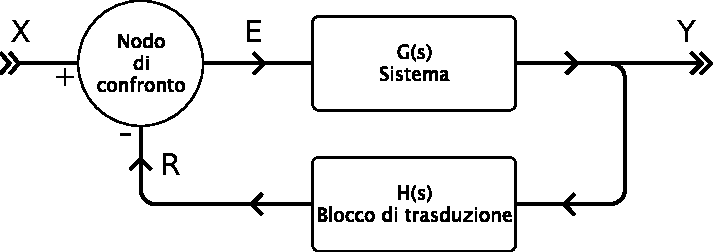
\includegraphics[width=.5\textwidth]{../E06/latex/s2.pdf}
\caption{Schema logico del sistema di controllo proporzionale di temperatura.}
\label{fig6:scheme2}
\end{wrapfigure}

Aggiungiamo ora al circuito proposto nel paragrafo precedente un sistema di controllo proporzionale, la cui funzione sarà quella di riscaldare una resistenza fino a raggiungere una data temperatura di soglia.

Per comprenderne meglio l'implementazione, generalizziamo prima il concetto di controllo proporzionale.
Osserviamo lo schema in Figura \ref{fig6:scheme2}: dati due segnali in ingresso X e R , il sistema deve rispondere con Y  se viene rispettata una condizione controllata dal nodo di confronto.
Quest'ultimo avrà dunque il compito di confrontare X ed R e verificare che la condizione, in generale funzione dei due segnali, sia rispettata.
L'aggiornamento di tale condizione è invece affidato al blocco di retroazione, che varia R.

Nel nostro caso, X è la tensione relativa alla temperatura di soglia ($T_{S}$) e R la tensione relativa alla temperatura misurata dalla termoresistenza ($T$).
La nostra Y sarà una data potenza dissipata su una resistenza di potenza che, se posta vicino alla PT100, ne varierà il valore di resistenza e quindi la temperatura letta dal circuito.
Dobbiamo ora identificare i blocchi relativi al sistema di controllo proporzionale e progettare quelli mancanti al circuito attuale.

Affidiamo il compito del blocco di retroazione al circuito finora costruito: questo restituisce un valore di tensione proporzionale alla temperatura letta dalla termoresistenza, che dovrà essere confrontato con la soglia.
Successivamente, il blocco di controllo deve fare la differenza fra questi due valori e, una volta raggiunto un valore impostabile, diminuire il valore della corrente fornita alla resistenza di potenza in maniera proporzionale ad E.
Definiamo dunque E=X-R, e per effettuare tale operazione utilizziamo un amplificatore differenziale.
Infine, per fornire la corrente necessaria alla resistenza, utilizzeremo un transistor BJT.
\vspace{-2mm}
\subsubsection{Confronto [Blocco 4]}

\begin{wrapfigure}[13]{r}{0.37\textwidth}
\centering
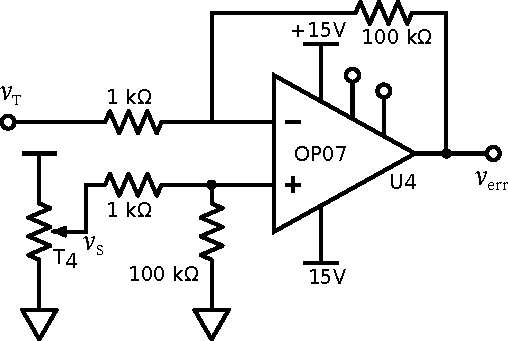
\includegraphics[width=.33\textwidth]{../E06/latex/P4.pdf}
\caption{Blocco di confronto}
\label{fig6:blocco4}
\end{wrapfigure}

Analizziamo il blocco di confronto proposto in Figura \ref{fig6:blocco4}.
Con il trimmer impostiamo una tensione $V_{S}$ proporzionale a $T_{S}$ (bisogna rispettare l'output del circuito precedente per impostarla, cioè $T_S = \frac{V_S}{\SI{100}{\milli\volt\per\celsius}}$) che può essere confrontata direttamente con la tensione $V_{T}$ relativa a $T$ in arrivo dal blocco di retroazione.
Inoltre, ponendo le resistenze uguali a \SI{1}{\kilo\ohm} e \SI{100}{\kilo\ohm} nel circuito di retroazione dell'amplificatore come in Figura, otteniamo un guadagno $G=100$.

Definendo la tensione in uscita dall'operazionale come $V_{err}$ e
$$\Delta T = \frac{|V_{S}-V_{T}|}{\SI{100}{\milli\volt}/\si{\celsius}}= | T_S - T | $$
Ovviamente, per valori di tensione in entrata maggiori di $\approx \SI{.15}{\volt}$, l'opamp entrerà in saturazione, mandando $V_{err}\approx \SI{15}{\volt}$; altrimenti l'amplificazione sarà quella di un amplificatore invertente.
Dunque varrà la seguente equazione (per $\Delta V = |V_S - V_T|$)

\begin{equation}
V_{err} = \bigg \{
\begin{array}{rl}
G \,\Delta V = G \,\Delta T \,\SI{100}{\milli\volt}/\si{\celsius}  & \mathrm{se} \quad 0<\Delta V<0.15 \si{\volt} \\
V_{U4}^{sat}\approx 15 \si{\volt} & \mathrm{se} \quad \Delta V>0.15 \si{\volt} \\
\end{array}
\label{eq6:exit_opamp}
\end{equation}

\subsubsection{Sistema [Blocco 5]}

\begin{wrapfigure}[17]{r}{0.2\textwidth}
\centering
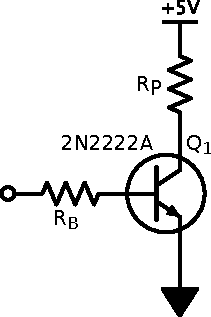
\includegraphics[height=5cm]{../E06/latex/P5.pdf}
\caption{Sistema di riscaldamento proporzionale}
\label{fig6:sistema}
\end{wrapfigure}

Per progettare il sistema di riscaldamento proporzionale, dobbiamo fornire potenza (ad una resistenza capace di dissipare molta energia e quindi di sopportare alti valori di corrente, detta \textit{resistenza di potenza}) in maniera proporzionale ad E, cioè $\Delta T$.
Per fare ciò, utilizzeremo un transistor 2N2222A con emettitore collegato a comune, le cui caratteristiche sono le seguenti
%$$\begin{array}{rl}
%\beta = \frac{I_c}{I_b} = 75\\
%V_{CE}^{sat}=0.4 \si{\volt}\\
%V_{BE}^{pol}=1.3 \si{\volt}\\
%\end{array}$$
$$\beta=\frac{I_c}{I_b}=75 \qquad V_{CE}^{sat}=\SI{.4}{\volt} \qquad V_{BE}^{pol}=\SI{1.3}{\volt}$$
Vale che, con una resistenza di potenza $R_{P} = \SI{27}{\ohm}$ e impostata una tensione di $5$ \si{\volt} costante ad uno dei suoi capi\footnote{Il REF02 non avrebbe potuto erogare la corrente necessaria a mantenere invariata la tensione ai capi della resistenza.
Dunque, per gestire questa tensione, abbiamo utilizzato il generatore di tensione costante Agilent E3631A.
Inoltre, per questo motivo, la comune utilizzata per questo blocco è stata posta indipendentemente per poi essere collegata a quella degli altri blocchi.} come in Figura \ref{gr6:proporzionale},
$$I_{C}=\frac{5 \si{\volt}- V_{CE}^{sat}}{R_P}=170 \si{\milli\ampere}$$
quindi $I_B=I_{C}/\beta=\SI{2.27}{\mA}$, da cui otteniamo il valore per cui il transistor si trova in saturazione (cioè quando la tensione base emettitore è pari a $V_{BE}^{pol}$ e la tensione base collettore è uguale a $V_{CE}^{sat}$)
$$R_B=\frac{V_{err} - V_{BE}^{pol}}{I_B}=2.2 \si{\kilo\ohm}$$

Considerando il seguente sistema che descrive il transistor e le resistenze calcolate in precedenza
$$
V_{err} = \begin{cases}
\begin{array}{rl}
\SI{5}{\volt}-V_{CE}^{sat} \geq \SI{5}{\volt}-V_{CE} = I_{C}R_P\\
I_C=\beta I_B \\
V_B - V_E = V_{BE} \leq V_{BE}^{pol} = V_{BE}^{sat}\\
V_{err}-V_B=I_B R_B
\end{array}
\end{cases}
$$
si può ottenere la condizione di saturazione come una condizione su $V_{err}$
\begin{equation}
V_{err}^{sat} \geq \frac{5\si{\volt}-V_{CE}^{sat}}{\beta} \frac{R_B}{R_P}+V_{BE}^{sat} \cong 6.3 \si{\volt}
\label{eq6:saturazione}
\end{equation}
e una condizione di interdizione (data da $I_C = 0 \Rightarrow I_B = I_C / \beta = 0$)
\begin{equation}
V_{err}^{int} = I_B R_B + V_B = V_B \leq V_{BE}^{pol} = \SI{1.3}{\V}
\label{eq6:interdizione}
\end{equation}
Per tensioni superiori a $V_{err}^{sat}$ il transistor sarà in zona di saturazione, per tensioni inferiori a $V_{err}^{int}$ sarà in interdizione e nella regione intermedia esso sarà governato linearmente dalla corrente di base.

Dunque, date (\ref{eq6:exit_opamp}), (\ref{eq6:saturazione}) e (\ref{eq6:interdizione}), il massimo della corrente e quindi, per la legge di Joule, il massimo della potenza dissipata da $R_P$ si avrà per $\Delta T \gtrsim 0.63 \si{\celsius}$), mentre il nostro circuito disabiliterà l'alimentazione della resistenza interdicendo il transistor per $\Delta V \lesssim \SI{.13}{\V}$, cioè quando la temperatura ambientale si porterà entro $\approx \SI{0.13}{\celsius}$ da $T_{S}$.


Ad un siffatto sistema abbiamo inoltre aggiunto un LED in modo tale che fosse acceso quando la resistenza $R_P$ fosse alimentata e fosse spendo quando il transistor fosse interdetto.
Per raggiungere tale scopo il diodo è stato messo in serie ad una resistenza da \SI{500}{\ohm} su un ramo parallelo alla resistenza di potenza $R_P$ affinché vi scorresse una corrente di circa \SI{10}{\mA}.
Tale particolare si può osservare nello schema circuitale in Figura \ref{gr6:proporzionale}.

\begin{figure}[ht]
 \centering
   {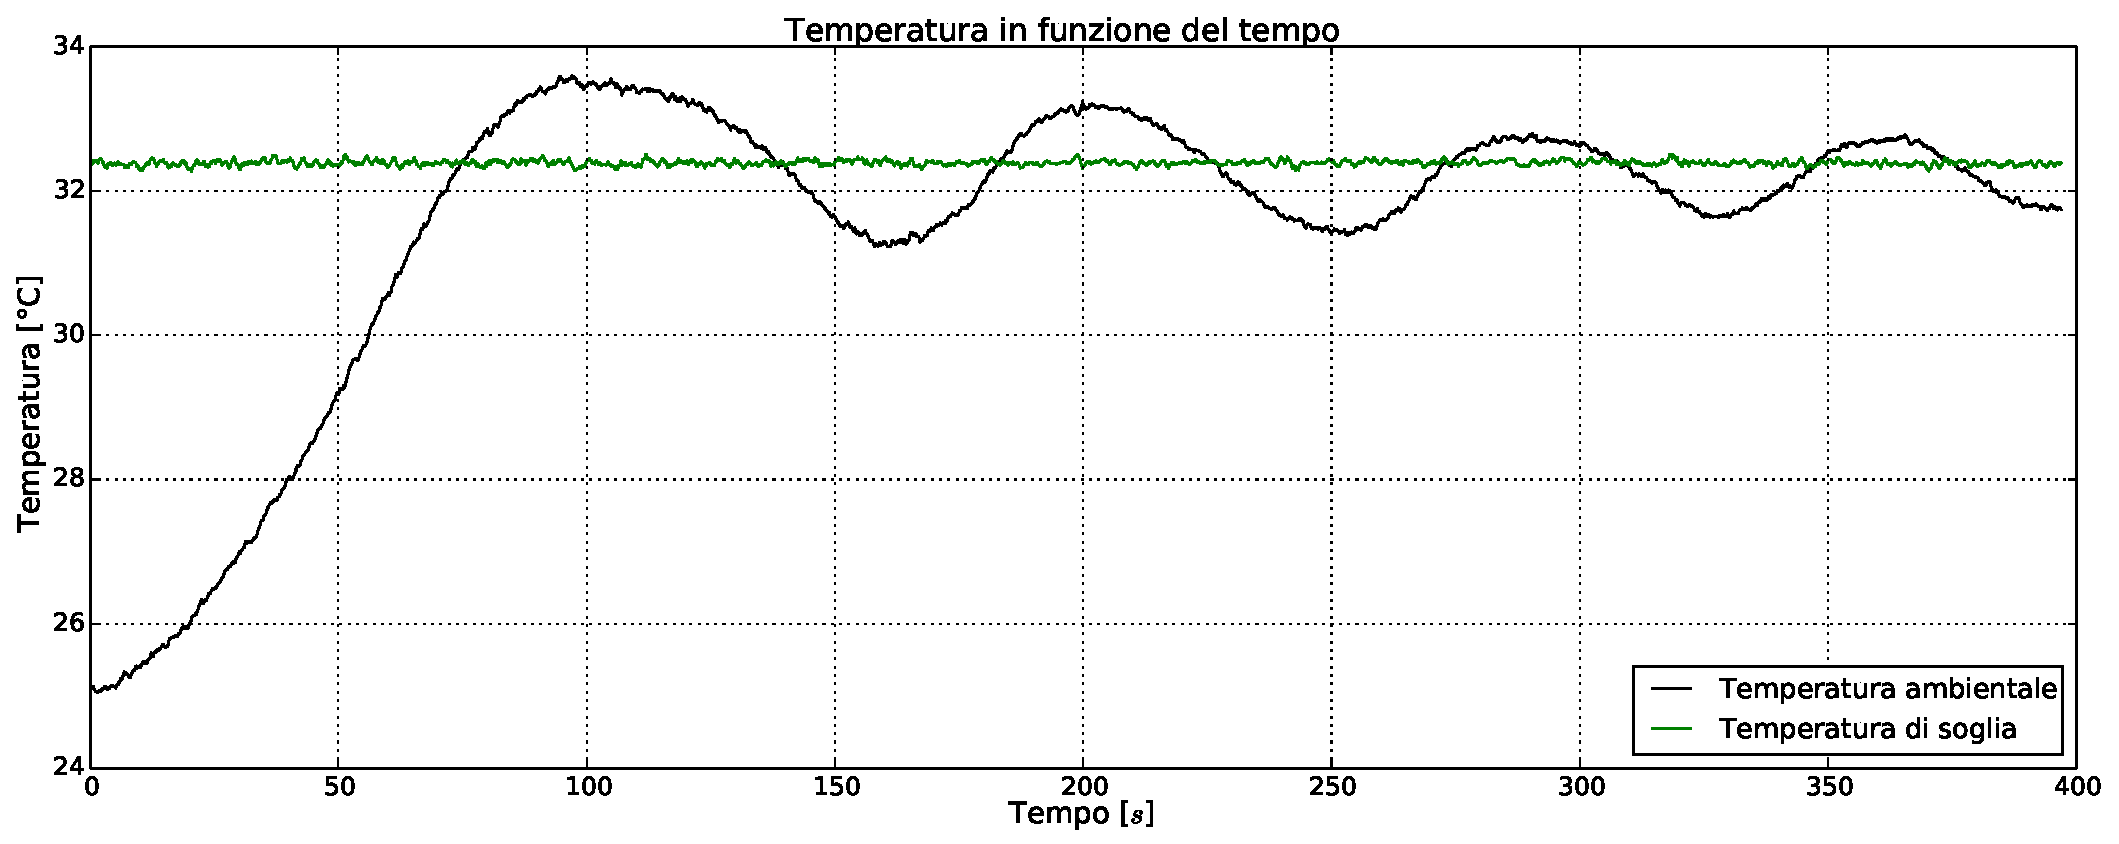
\includegraphics[width=1\textwidth]{../E06/latex/grafico.pdf}}
 \caption{Il grafico riporta la temperatura misurata dalla termoresistenza (in nero) e la temperatura di riferimento (in verde). Come si può osservare la temperatura di riferimento ha una certa instabilità data dall'instabilità della tensione all'ingresso non invertente dell'opamp nel blocco 4. L'imperferzione di tale segnale è probabilmente imputabile non all'integrato REF02, bensì a rumori ambientali.}
 \label{gr6:grafico}
\end{figure}

\begin{figure}[htc!]
 \centering
   {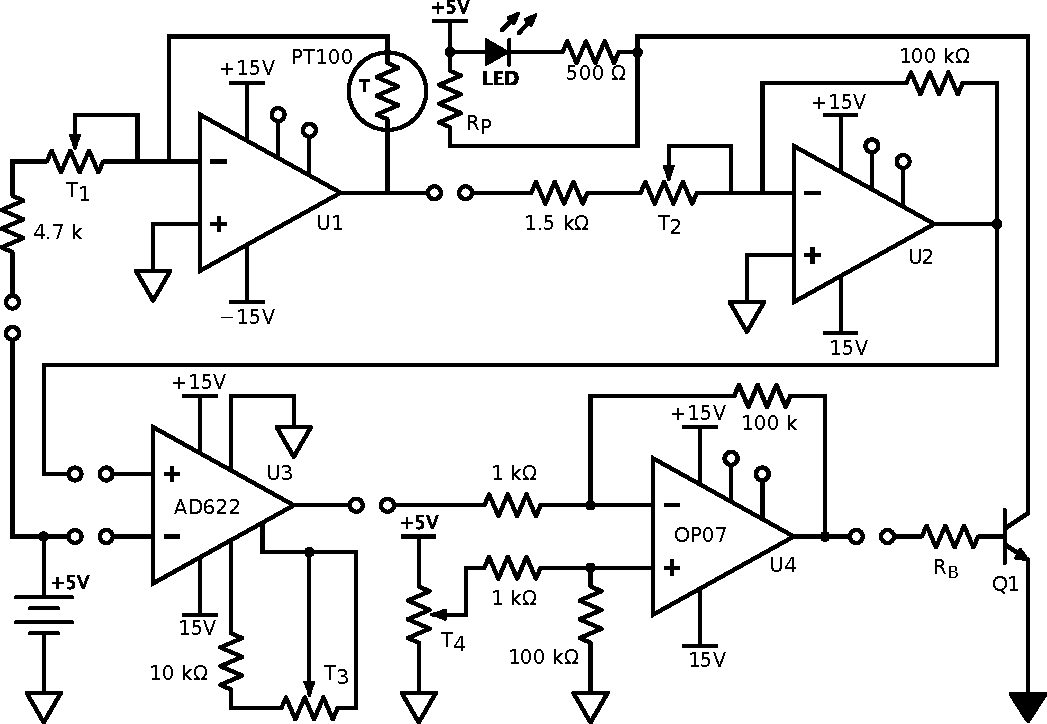
\includegraphics[width=0.78\textwidth]{../E06/latex/c2.pdf}}%.75
 \caption{Schema circuitale del sistema di controllo proporzionale della temperatura composto di un termometro elettronico e di un sistema di riscaldamento.}
 \label{gr6:proporzionale}
\end{figure}
